\chapter{Meshless methods} \label{chap:meshless_methods}

Meshless or Meshfree Methods (MMs) were developed to overcome the drawbacks of traditional mesh-based methods for the solution of Partial Differential Equations (PDE), where their true advantage is that ``the approximation of unknowns in the PDE is constructed based on scattered points without mesh connectivity''~\cite{Chen:meshless_overview_after_20_years}. The conceptual difference between Mesh Based and Meshless methods can be visualized on figure~\ref{fig:mesh_vs_meshless}: the former patch the domain with some geometrical shapes while the latter only distributes nodes across the domain.

\begin{figure}
	\centering
	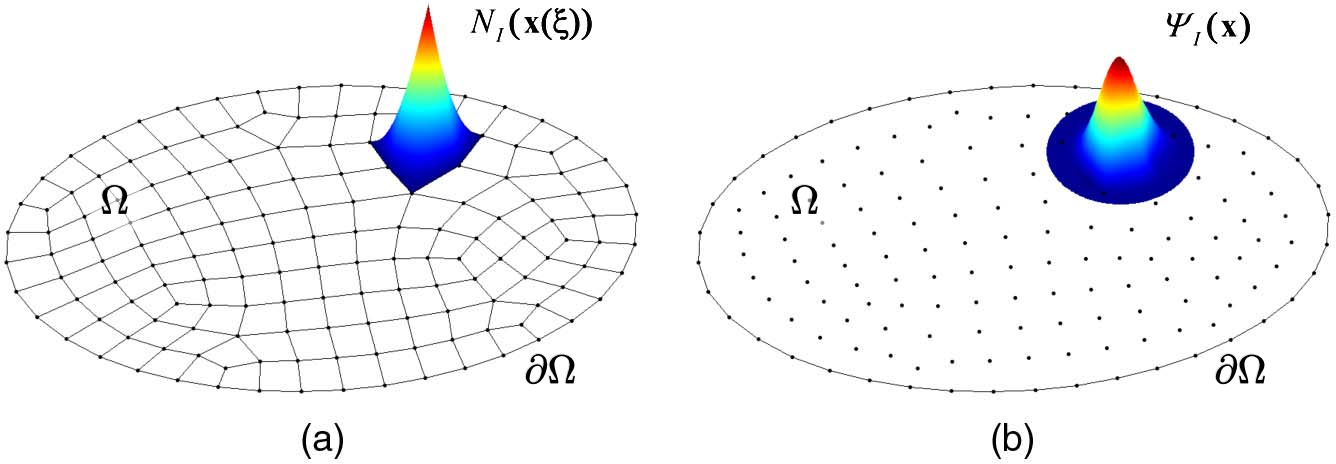
\includegraphics[width=\textwidth]{img/mesh_vs_meshless.png}
	\caption{$(a)$ Example of reconstruction of a PDE solution, via mesh based method, for a single finite element domain; $(b)$ approximation of the same function obtained through meshless approach. Figure taken from~\cite{Chen:meshless_overview_after_20_years}}
	\label{fig:mesh_vs_meshless}
\end{figure}

They appeared for the first time in $1977$ with the Smooth Particle Hydrodynamics (SPH) method~\cite{Belytschko:meshless_overview}, initially used to modeling astrophysical phenomena such as exploding stars and dust clouds was later applied in solid mechanics to overcome limitations of mesh-based methods~\cite{Benz:SPH_on_solid_mechanics}. To improve accuracy, tensile instability and spatial instability of SPH, many more modern MMs have been developed: the introduction of Reproducing Kernel Particle Method (RKPM)~\cite{Liu:RKPM} is a prime example of enhanced consistency and stability.
Generalized Finite Difference (GFD) methods is another branch of numerical methods for solving PDEs that do not rely on a grid structure and many modern MMs originate from the employment of this approximation for solving PDEs.
%TODO: Aggiungi chi ha introdotto i GFD??

The typical use case for MMs is the construction of an approximating field $u^{h}$ for the sought solution $u\colon\Omega\subset \R^{d}\to\R$ of the following boundary value problem:
\begin{equation}
	\label{eqn:generic_continous_PDE}
	\begin{cases}
		\mathcal{L} u(\vec{x})  = f(\vec{x})		& \text{in $\Omega$} \\
		\mathcal{B} u(\vec{x})   = g(\vec{x})	     & \text{on $\partial\Omega$}
	\end{cases}
\end{equation}
where $\mathcal{L}$ is a generic linear differential operator and $\mathcal{B}$ is a different linear operator used to enforce some Boundary Condition (BC) that does not necessarily involves partial derivatives; $f$ and $g$ are known functions.
Usually in the Computational Fluid Mechanics (CFD) world the encountered BC are:
\begin{align}
	& \text{Dirichlet BC:} & u=g  \\
	& \text{Neumann BC:} & \frac{\partial u}{\partial \vec{n}} = g  \\
	& \text{Robin BC:} & au + b\frac{\partial u}{\partial \vec{n}} = g
\end{align}
where $\partial u / \partial \vec{n}$ indicate the normal derivative of $u$ along the surface normal whereas $a$ and $b$ are known functions. It can also be noticed that Dirichlet and Neumann BCs are special cases of Robin BC respectively when $b(\vec{x})=0$ and $a(\vec{x})=0$.

%TODO: Aggiungi il fatto che l'approx è necessaria per ricavare i valori numerici
Regardless on the Meshfree approach, the following approximation for any solution $u$ can be written:
\begin{equation}
	\label{eqn:general_u_discretization}
	u^{h}(\vec{x}) = \sum_{k= 1}^{N} {\alpha_k B_k(\vec{x})}
\end{equation}
where $B_k\colon\Omega\to\R$ are suitable basis functions and $\alpha_k$ are the expansions coefficients that must be determined.
% Meglio considerare dominio come Omea + partialOmega??
Different choices for the basis functions $B_k$ leads to different formulations and in literature can be found several of these, some examples are: RKPM~\cite{Liu:RKPM}, moving least square (MLS)~\cite{Lancaster:MLS}, radial basis function (RBF)~\cite{Kansa:RBF_1, Kansa:RBF_2} and partition of unity (PU)~\cite{Schweitzer:PU}. Furthermore solving the PDE in~\eqref{eqn:generic_continous_PDE} with the approximated solution $u^h$, in general, yields to a non-zero error function $\epsilon^{h}$ given by:
\begin{equation}
	\epsilon^{h}(\vec{x}) = \mathcal{L} u^{h}(\vec{x}) - f(\vec{x})
\end{equation}

Once the general form of the approximated solution in~\eqref{eqn:general_u_discretization} has been properly defined, it can be employed for discretizing the PDE, reported in~\eqref{eqn:generic_continous_PDE}, over a set of N generated nodes $\Set{\vec{x}_1, \dots, \vec{x}_N}$ distributed in the physical domain $\Omega \cup \partial\Omega$.
% Vuoto sul cosa siano queste test function Gamma...
The Weighted Residual Method is used to do so: a set of test functions $\Set{\Gamma_1, \dots, \Gamma_N}$ orthogonal to $\epsilon^{h}$ are used to integrate the error to zero:
\begin{equation}
\label{eqn:constraints_to_integrate_MMs_errors_to_zero}
	\begin{split}
		\int_{\Omega} \Gamma_i \epsilon^{h}\,d\Omega & = \int_{\Omega} \Gamma_i (\mathcal{L} u^{h}(\vec{x}) - f(\vec{x}))\,d\Omega  \\
		& = \int_{\Omega} \Gamma_i \Bigl[ \mathcal{L}\Bigl( \sum_{k= 1}^{N} {\alpha_k B_k(\vec{x})}\Bigr) - f(\vec{x})\Bigr]\,d\Omega = 0
	\end{split}
\end{equation}
where $i=1, \dots, N$. From the choice of functions $\Gamma_i$ the following two formulations are obtained~\cite{Chen:meshless_overview_after_20_years}:
\begin{description}
	\item[Galerkin Meshless Methods] that find a weak solution for the PDE by using as test functions the basis functions $B_k$. These formulations require domain integration and special techniques to enforce boundary conditions;
	\item[Collocation Meshless Methods] that find a strong solution for the PDE by using Dirac delta functions centered at the discretization nodes as test functions. Basically they enforce equaitons~\eqref{eqn:generic_continous_PDE} on a finite set of nodes, and by doing so, they do not require any domain integration.
\end{description}

Finally, once constraints~\eqref{eqn:constraints_to_integrate_MMs_errors_to_zero} are enforced, the solution of problem~\eqref{eqn:generic_continous_PDE}, i.e. the values $\Set{u^h(\vec{x}_1), \dots, u^h(\vec{x}_N)}$, can be found solving the linear system  resulting from PDE's discretization. We remark that the system obtained is not linear in general, but it is in this case since the PDE is linear. Nevertheless, also non-linear PDEs can be reduced to the aforementioned case thanks to a proper linearization.

%\section{Motivation of case study}

%\section{RBF-FD method}
%
%In this section we explain in more details the MM used within this work: the Radial Basis Function generated Finite Differences (RBF-FD) method. To do so we consider a physical domain $\Omega \cup \partial\Omega \subset \R^d$ indicating with $\Omega$ the open subset, $\partial \Omega$ its boundary and with $d \in \N$ its dimension; over the presented domain we define a boundary value problem with the same form of the one reported in~\eqref{eqn:generic_continous_PDE} and we show how RBF-FD method can be used to solve it.
%
%% Aggiungere qualche riga sull'importanza dellla distribuzione dei punti??
%As any other MM, before starting, a set of $N$ points distributed over the domain where to discretize the PDE is required. We indicate it with $\mathcal{X} := \Set{\vec{x}_1, \dots,  \vec{x}_N \mid \vec{x_i} \in \Omega\cup\partial\Omega, \, i=1, \dots, N}$. To remark also the fact that nodes are placed both inside the domain and on its boundary we partition $\mathcal{X}$ in $\mathcal{X_I}$, the set of internal nodes, and $\mathcal{X_B}$, the set of boundary nodes, defined as:
%\begin{gather*}
%	\mathcal{X_I} := \Set{\vec{x}_1, \dots,  \vec{x}_{N_I} \mid \vec{x}_i \in \Omega, \, i=1, \dots, N_I} \\
%	\mathcal{X_B} := \Set{\vec{x}_1, \dots,  \vec{x}_{N_B} \mid \vec{x}_i \in \partial\Omega, \, i=1, \dots, N_B}
%\end{gather*}
%where $N_I$ and $N_B$ indicate respectively the number of nodes inside and on the boundary. Of course $N_I + N_B = N$ and $\mathcal{X_I} \cup \mathcal{X_B} = \mathcal{X}$.
%
%This method, like other MMs, looks for an approximated solution of problem~\eqref{eqn:generic_continous_PDE} in the form of~\eqref{eqn:general_u_discretization}.
%
%%Radial Basis Function generated Finite Differences (RBF-FD) method, as any other MM, is used to solve approximately PDEs via scattered data interpolation. In particular, to do so, it makes use of the FD to define an approximation of partial derivatives for PDEs solution.
%
%\subsubsection{RBF Interpolation}
%Every MM, as we have already seen, on its core, is just a way to approximate the solution of a PDE and RBF-FD method is no exception. The tool used to do so is called scattered data interpolation and in this subsection, after explaining what it is, we see how it is related to the solution of problem~\eqref{eqn:generic_continous_PDE}.  During the explanation we start by seeing how it is used in general by MMs so to avoid becoming fixated on a single implementation and losing generality, furthermore this way of proceeding establishes all the steps that are also used in case of RBF basis functions.
%%[Metti qui il discorso dell'interpolazione locale o globale??]
%% Aggiungi un recall al problema??
%
%In general, given the set of nodes $\mathcal{X}$, and a set of known real values $u(\vec{x}_1), \dots, u(\vec{x}_N)$, the interpolation problem results on finding a continuous function $u^{h} \colon \Omega\subset\R^{d} \to \R$ that satisfy:
%\begin{equation}
%	\label{eqn:interpolation_constraints}
%	u^{h}(\vec{x_i}) = u(\vec{x}_i) \qquad  \forall \vec{x}_i \in \mathcal{X}
%\end{equation}
%
%MMs also aim to provide an approximation for an unknown function, but in addition give an hint on its form as reported in equation~\eqref{eqn:general_u_discretization}, without further specifying the coefficients values. We report here its definition for conveniency:
%\begin{equation}
%	\label{eqn:general_u_discretization_RBF_section}
%	u^{h}({x}) = \sum_{k= 1}^{N} {\alpha_k B_k(\vec{x})}
%\end{equation}
%Here is where the theory of scattered data interpolation comes in: it tells us that we are able to find the numerical values for $\alpha_1, \dots \alpha_N$ if we impose a number of conditions equal to the number of coefficients that we are looking for. These conditions must have a form like that shown in equation~\eqref{eqn:interpolation_constraints}. Therefore if we replace the generic meshless approximation within each of the $N$ interpolation conditions we can write the following system of linear equation:
%\begin{equation}
%\label{eqn:general_system_from_scattred_data_interpolation}
%	\underbrace{
%		\begin{bmatrix}
%			B_1(\vec{x}_1)  & \dots		& B_N(\vec{x}_1)     \\
%			\vdots					& \ddots  & \vdots					      \\
%			B_1(\vec{x}_N)  & \dots		& B_N(\vec{x}_N)
%		\end{bmatrix}}_{\boldsymbol{B}}
%\begin{bmatrix}
%	\alpha_1 \\
%	\vdots		\\
%	\alpha_N
%\end{bmatrix}
%=
%\begin{bmatrix}
%	u(\vec{x}_1)  \\
%	\vdots				\\
%	u(\vec{x}_N)
%\end{bmatrix}
%\end{equation}
%that, once solved, provides us with the desired coefficients that make up $u^h$.
%We would like to stress the fact that the right hand side vector is made up of values of the unknown exact solution of problem~\eqref{eqn:generic_continous_PDE}, that we only \textit{assume } to know.
%
%For solving problem~\eqref{eqn:generic_continous_PDE} (we refer to~\cite{Liu:Intro_to_meshfree_methods} for a detailed explanation) the following constraints are enforced instead:
%\begin{equation}
%	\begin{aligned}
%		\mathcal{L} u^h(\vec{x}_j) = f(\vec{x}_j) \quad & \text{if $\vec{x}_j \in \Omega$}  \\
%		u^h(\vec{x}_j) = g(\vec{x}_j) 						    \quad & \text{if $\vec{x}_j \in \partial\Omega$}
%	\end{aligned}
%\end{equation}
%and granting that first $N_I$ nodes belongs to $\Omega$ and the last $N_B$ to $\partial\Omega$, we can find the values of the approximated solution at the points in $\mathcal{X}$ by solving:
%\begin{equation}
%\begin{bmatrix}
%	c_{1,1} 		& 	\dots 		& c_{1,N_I}  \\
%	\vdots			& \ddots	& \vdots		\\
%	 c_{N_I,1} & \dots		& c_{N_I,N_I}
%\end{bmatrix}
%\begin{bmatrix}
%	u^h(\vec{x}_1)  \\
%	\vdots					\\
%	u^h(\vec{x}_{N_I})
%\end{bmatrix}
%=
%\boldsymbol{f} -
%\begin{bmatrix}
%	c_{1,N_I+1} 		& 	\dots 		& c_{1,N_B}  \\
%	\vdots			& \ddots	& \vdots		\\
%	c_{N_I,N_I+1} & \dots		& c_{N_I,N_B}
%\end{bmatrix}
%\boldsymbol{g}
%\end{equation}
%where $\boldsymbol{f} = [f(\vec{x}_1) \dots f(\vec{x}_{N_I})]^T$ and $\boldsymbol{g} = [g(\vec{x}_{N_I+1}) \dots g(\vec{x}_{N_B})]^T$, and the coefficient matrix $\boldsymbol{C}$ is found as the solution of:
%\begin{equation}
%\label{eqn:generic_discretized_PDE_by_MMs}
%\begin{bmatrix}
%	c_{1,1} 		& 	\dots 		& c_{N_I,1}  \\
%	\vdots			& \ddots	& \vdots		\\
%	c_{1,N} & \dots		& c_{N_I,N}
%\end{bmatrix}
%=
%\boldsymbol{B}^{-T}
%\begin{bmatrix}
%	\mathcal{L} B_1(\vec{x}_1)  & \dots		& \mathcal{L} B_1(\vec{x}_{N_I})     \\
%	\vdots												& \ddots  & \vdots					      								  \\
%	\mathcal{L} B_N(\vec{x}_1)  & \dots		& \mathcal{L} B_N(\vec{x}_{N_I})
%\end{bmatrix}
%\end{equation}
%By carefully analyzing each row $\boldsymbol{c}_i = [c_{i,1}, \dots c_{i,N}]$ of matrix $\boldsymbol{C}$ we can notice that are computed solving the following linear systems:
%\begin{equation}
%	\boldsymbol{B}^T c_i = 
%	\begin{bmatrix}
%		\mathcal{L} B_1(\vec{x_i})  \\
%		\vdots											  \\
%		\mathcal{L} B_N(\vec{x_i})
%	\end{bmatrix}
%\qquad i=1, \dots, N_I
%\end{equation}
%which are closely related to the one obtained from scattered data interpolation reported in~\eqref{eqn:general_system_from_scattred_data_interpolation} due to the presence of the same matrix $\boldsymbol{B}$. We conclude by commenting that equation~\eqref{eqn:generic_discretized_PDE_by_MMs} with matrix $\boldsymbol{B}$ defined as in~\eqref{eqn:general_system_from_scattred_data_interpolation} holds true only in case of Dirichlet boundary conditions, otherwise $\boldsymbol{B}$ would take on a different form.
%
%In the case of RBF-FD method the implementation of scattered data interpolation and the solution of governing equation remain the same and leads to a matrix $\boldsymbol{B}$ defined as:
%\begin{equation}
%\boldsymbol{B} =
%\begin{bmatrix}
%	\Phi(\vec{x}_1, \vec{x}_1)  & 	\dots 	& 	\Phi(\vec{x}_1, \vec{x}_N)  \\
%	\vdots											& \ddots &  \vdots											  \\
%	\Phi(\vec{x}_N, \vec{x}_1)  & 	\dots 	& 	\Phi(\vec{x}_N, \vec{x}_N)
%\end{bmatrix}
%\end{equation}
%
%\subsubsection{Radial Basis Functions} \label{subsec:radial_basis_functions}
%Radial Basis Functions (RBFs) are the basis functions used in~\eqref{eqn:general_u_discretization} by the RBF-FD method to approximate the solutions of PDEs and are defined as:
%\begin{equation}
%	\label{eq:RBF_definition}
%	\Phi_k(\vec{x}) = \varphi(\norm{\vec{x} - \vec{x}_k}_2)
%\end{equation}
%where $\vec{x}_k \in X$ is a given point , $\norm{\cdot}_2$ is the euclidean distance and $\varphi\colon \Omega\cup\partial\Omega \to \R$, named basic function, is a scalar field which takes $\vec{x}$ as input and it is used as generator for all the basis functions. In general different basic functions $\varphi$ can be used, some of them are reported in table~\ref{tab:basic_functions}.
%
%To further clarify the RBFs name we can notice that they are called:
%\begin{description}
%	\item[Radial] since the value of each $\phi_k{(\vec{x})}$ at each point $\vec{x}$ depends only on the distance between that point and $\vec{x}_k$ through $\norm{\cdot}_2$, they satisfy radial symmetry;
%	\item[Basis] since the set of radial functions $\phi_k{(\vec{x})}$ with $k=1, \dots, N$ form a basis for the space of functions:
%	\[
%	F_{\Phi} := \Set{ \sum_{k=1}^{N} \alpha_k \Phi_k{(\vec{x})},  \quad \alpha_k \in\R }
%	\]
%\end{description}
%
%\begin{table}
%	\caption{Examples of basic functions where $r_k = \norm{\vec{x} - \vec{x}_k}_2$ and $\epsilon$, called shape factor, is a suitable parameter}
%	\label{tab:basic_functions}
%	\centering
%	\begin{tabular}{cc}
%		\toprule
%		Name										&  $\varphi(r_k)$																	\\
%		\midrule
%		Multiquadratic					  &  $\sqrt{1 + ( 1 + \epsilon r_k)^2}$										\\
%		Inverse multiquadratic	 &  $\big(  \sqrt{1 + ( 1 + \epsilon r_k)^2}  \big)^{-1}$  \\
%		Thin plate splines			   &  $r_k^l \log r_k, \, l  \, \text{even}$								\\
%		Gaussian							    &  $e^{- (\epsilon r_k)^2}$												  \\
%		Polyharmonics					&  $r_k^l, \, l  \, \text{odd}$														\\
%		\bottomrule
%	\end{tabular}
%\end{table}
%
%\subsubsection{The Mairhuber-Curtis Theorem}
%
%From the previous discussion, in particular from equation~\eqref{eqn:generic_discretized_PDE_by_MMs}, it can be noticed that matrix $\boldsymbol{B}$ has to be non singular in order to be able to solve the boundary value problem, and this must hold for each node placement $\mathcal{X}$ (to be read as every possible discretization of the problem domain) as long nodes are distinct. This property of $\boldsymbol{B}$ turns out to be dependent on the choice of the particular set of basis functions: for example if we assume $B_k(\vec{x})\in\Pi_P^d$ and $\Set{B_1(\vec{x}), \dots, B_N(\vec{x})}$ to be a polynomial basis of the space $\Pi_P^d$ of polynomials of degree at most $P$ in $\R^d$, then we are not able to guarantee that $\vec{B}$ is invertible for $d>1$.
%
%This issue is explained in more detail by the Mairhuber-Curtis theorem~\cite{Mairhuber:interpolation_basis_problem}; when dealing with the multidimensional case it is possible to continuously move two nodes such that they end up by interchanging their original positions without one crossing the path of the other. If these $2$ are the only nodes of $\mathcal{X}$ that are moved, $\boldsymbol{B}$ ends up with $2$ rows exchanged leading to a change in the sign of its determinant, and, since the determinant is a continuous function, this means that there is a moment when the latter vanishes making the matrix singular.
%
%The inconvenience arises from the fact that the set of basis functions is independent from the node position and could be solved by simply choosing a basis that is function of nodes position. By doing so we no more fall in the case of the Mairhuber-Curtis theorem since whenever we move nodes also the base itself changes and if two nodes switches their positions not only their respective rows in $\boldsymbol{B}$ are switched, but also their columns, forcing the determinant not to change in sign.
%
%%TODO: Say something about the suitable node generation algorithm and then tells about polynomial augmentation and why it is required (see Riccardo thesis?). Once you've done that you can continue and start talking about RBF.
%
%\subsubsection{Polynomial augmentation}
%
%Setting aside the issue of the invertibility of matrix $\boldsymbol{B}$ in case of particular nodes arrangement discussed in previous subsection, we should also take into account  the accuracy of the interpolation that we're able to achieve, which also depends upon the type of functions that we are supposed to aprroximate.
%%[\textbf{Qui c'è una vecchia versione]}
%%In the previous subsection we have seen that we are able to obtain a unique (thanks to the non singularity of matrix $\vec{B}$ ensured by proper usage of RBFs) interpolant $g$ satisfying interpolation constraints~\eqref{eqn:interpolation_constraints}. 
%%
%%What is lacking in our discussion is the level of accuracy that we are able to reach which also depends upon the type of function that we are supposed to interpolate.
%Indeed RBFs approximation schemes alone are not able to interpolate constant, linear or higher degree polynomials fields and this is an issue since they are important in different engineering applications such modeling of constant strain in elastic bodies and steady temperature fields in differentially heated walls~\cite{Zamolo:phd_thesis}.
%
%To overcome this limitation a polynomial augmentation of degree $P$ is required, leading to the overall formulation for the RBF interpolant:
%\begin{equation}
%	\label{eq:RBF_interpolator_plus_polynomial_augmentation}
%	u^h(\vec{x}) = \sum_{j=1}^{N} \alpha_j \Phi_k(\vec{x}) + \sum_{k=1}^{M} \beta_k p_k(\vec{x})
%\end{equation}
%where $M=\binom{P+D}{D}$ is the number of polynomial basis functions with degree $P \le D$, $\Set{p_1(\vec{x}) \dots p_M({\vec{x}})}$ is a complete polynomial basis of $\Pi_P^d$ and $\beta_j$ are the corresponding coefficients to each function in the former basis. An example of polynomial basis for polynomials of degree $P=1$ in $2D$ has the following $M=3$ elements: $p_1(x,y) = 1$, $p_2(x,y) = x$, $p_3(x,y) = y$.
%
%We must also note that using an interpolant with the introduced polynomial augmentation, during the approximated solution of problem~\eqref{eqn:generic_continous_PDE} leads to an underdetermined system in~\eqref{eqn:general_system_from_scattred_data_interpolation}. In order to obtain a square $\vec{B}$ and thus having a solvable system, the following orthogonality conditions, that guarantees polynomial reproduction, have to be imposed:
%\begin{equation}
%	\label{eqn:orthogonality_conditions_for_square_B_in_case_of_poly_augmentation}
%	\sum_{i=1}^{N} \alpha_i p_k(\vec{x}_i) = 0, \qquad i=1, \dots, M
%\end{equation}
%The coefficients of $u^h$, which are now composed not only by $\vec{\alpha} = [\alpha_1 \dots \alpha_N]$, but also by $\vec{\beta} = [\beta_1 \dots \beta_M]$, can then be found by solving the following system:
%\begin{equation}
%\begin{bmatrix}
%	\vec{B}  & \vec{P}  \\
%	\vec{P}^T  & \vec{0}
%\end{bmatrix}
%\begin{bmatrix}
%	\vec{\alpha}  \\
%	\vec{\beta}
%\end{bmatrix}
%=
%\begin{bmatrix}
%	\vec{u}  \\
%	\vec{0}
%\end{bmatrix}
%\end{equation}
%where:
%\begin{equation}
%	\begin{aligned}
%		\vec{P} & =
%		\begin{bmatrix}
%			p_0(\vec{x}_1)  & \dots     & p_M(\vec{x}_1)  \\
%			\vdots					 & \ddots  & \vdots						\\
%			p_0(\vec{x}_N)  & \dots     & p_M(\vec{x}_N)  \\
%		\end{bmatrix}  \\
%		\vec{u} & = [u(\vec{x}_1). \dots u(\vec{x}_N)]
%	\end{aligned} 
%\end{equation}
%From its formulation is easy to understand that the system above is simply the composition of the system in equation~\eqref{eqn:general_system_from_scattred_data_interpolation}, first row, with constraints~\eqref{eqn:orthogonality_conditions_for_square_B_in_case_of_poly_augmentation} written in compact form, second row.
%
%In practice the addition of polynomial basis to the RBF interpolant let us perfectly fit $u(\vec{x})$ not only on collocation points where we have $u^h(\vec{x}_i)  = u(\vec{x}_i)$, but also across the rest of the domain provided that data $u(\vec{x}_1) \dots u(\vec{x}_N)$ come from a polynomial of total degree less than or equal to $P$.  Nevertheless this procedure has as a side effect since not all the basic functions $\varphi$ leads to a well-posed RBF interpolation with a non singular matrix $M$, but only the strictly conditionally positive definite of order $P+1$ ones.
%
%%TODO: Aggiungi reference alle conditionally positive definite


%[\textbf{Da qui in poi skippa che è una parte vecchia}]
%Combining them with equations~\eqref{eq:interpolation_system} and~\eqref{eq:RBF_interpolator_plus_polynomial_augmentation} we get:
%\begin{equation}
%	\left[
%	\begin{array} { c                             													| c }
%									\begin{array}{ccc}
%																	\varphi(\norm{\vec{x}_1 - \vec{x}_1}_2) & \dots & \varphi(\norm{\vec{x}_1 - \vec{x}_n}_2)  \\
%																	\vdots 																		& \ddots & \vdots																		 \\
%																	\varphi(\norm{\vec{x}_n - \vec{x}_1}_2) & \dots & \varphi(\norm{\vec{x}_n - \vec{x}_n}_2)\\
%									\end{array} &														\begin{array}{ccc}
%																																	p_1(\vec{x}_1)  &  \dots  & p_m(\vec{x}_1)  \\
%																																	\vdots					& \ddots & \vdots					  \\
%																																	p_1(\vec{x}_n)  &  \dots  & p_m(\vec{x}_n)
%																														  \end{array} \\
%																													
%									\hline
%									\begin{array}{ccc}
%										p_1(\vec{x}_1)  &  \dots  & p_m(\vec{x}_1)  \\
%										\vdots					& \ddots & \vdots					  \\
%										p_1(\vec{x}_n)  &  \dots  & p_m(\vec{x}_n)
%									\end{array} & 														\begin{array}{ccc}
%																																0 			  &  \dots     & 0  		\\
%																																\vdots  &  \ddots  & \vdots  \\
%																																0			  & \dots	   & 0
%																														  \end{array}
%								\end{array}
%	\right]
%	\begin{bmatrix}
%		\alpha_1  \\
%		\vdots		 \\
%		\alpha_n \\
%		\beta_1		\\
%		\vdots		 \\
%		\beta_m
%	\end{bmatrix} = 
%	\begin{bmatrix}
%		f_1  			 \\
%		\vdots		 \\
%		f_n 			\\
%		0				  \\
%		\vdots		 \\
%		0
%	\end{bmatrix}
%\end{equation}
%[sostituire $\varphi$ con $\varPhi$ o almeno fixare la formattazione dell'equazione]
%and its compact version using block matrix notation:
%\begin{equation}
%	\label{eq:RBF_interpolation_system_with_polynomial_augmentation}
%	\underbrace{\begin{bmatrix}
%		\vec{\varPhi} & \vec{P} \\
%		\vec{P}^T		 & \vec{0}
%	\end{bmatrix}}_{\vec{M}}
%\begin{bmatrix}
%	\vec{\alpha} \\
%	\vec{\beta}
%\end{bmatrix} = 
%\begin{bmatrix}
%	\vec{f} \\
%	\vec{0}
%\end{bmatrix}
%\end{equation}
%where $\vec{\varPhi}$ is a $(n \times n)$ square matrix with entries $\vec{\varPhi}_{ij} = \varphi(\norm{\vec{x}_i - \vec{x}_j}_2)$ is just the $\vec{B}$ matrix of equation~\eqref{eq:interpolation_system} with the RBFs instead of the generic ones, $\vec{P}$ is the $(n \times m)$ matrix associated to the polynomial basis, $\vec{\alpha} \in \R^n$ and $\vec{\beta} = [\beta_1, \dots, \beta_m]\in \R^m$ are the vectors  related to the $n+m$ unknowns. $\vec{f} \in \R^{n}$, instead, is the vector containing the known set of values given for the interpolation. Therefore if we want to compute the coefficients of our polynomial-augmented RBF interpolant we can simply solve for $[\vec{\alpha},\vec{\beta}]^{T}$ system~\eqref{eq:RBF_interpolation_system_with_polynomial_augmentation}.
%
%At this point someone might points out that matrix $\vec{M}$ is no more the same as $\vec{B}$ with RBFs as basis functions since we've added more columns and rows and so we are no more sure of the existence and uniqueness of $[\vec{\alpha},\vec{\beta}]^{T}$.  Although this observation is correct in general, we are able to guarantee the same properties of $\vec{B}$ also to $\vec{M}$ by properly choosing $\varphi$ in the RBF definition. The Multiquadratic function presented in table~\ref{tab:basic_function_examples} does this and in the following we assume to use that basic function. For more  details we refer to~\cite{Fasshauer:details_on_basic_functions}.

%TODO: Questa \subsection potrrebbe essere buona da spostare nel Chapter2.tex
%\subsection{RBF Method}
%So far we have talked about data interpolation and we ended up in the system of equation~\eqref{eq:RBF_interpolation_system_with_polynomial_augmentation} that can be employed for every interpolation problem of the form explained in subsection~\vref{subsec:radial_basis_functions}, now we make the next step and we explain how this method can be employed in the solution of PDEs.
%[\textbf{Da valutare se mettere qua il discorso dei nodi}]

%\subsection{Boundary conditions}
%Since in RBF-FD an RBF interpolator is used to find the solution of a generic PDE, like the~\eqref{eq:Poisson_equation} reported at the beginning of this section, we must take into account also of BCs during the interpolation. [Modifica la PDE usata nell'introduzione ai MMs]
%In order to satisfy them we need to split the interpolation conditions defined in equations~\eqref{eqn:interpolation_constraints} for the internal, $X_I$, and boundary, $X_B$, sets of points:
%\begin{subequations}
%	\begin{align}
%		g(\vec{x_i}) &=f_i \qquad  \forall \vec{x}_i \in X_I \\
%		\mathcal{B} \big( u^h(\vec{x}_i) \big) &= g(\vec{x}_i) \quad \forall \vec{x}_i \in X_B \label{eq:interpolation_constrs_for_Xb}
%	\end{align}
%\end{subequations}
%
%By writing more explicitly constraints~\eqref{eq:interpolation_constrs_for_Xb} using the interpolator in~\eqref{eq:RBF_interpolator_plus_polynomial_augmentation}:
%\begin{equation}
%	\sum_{k=1}^{N} a_k \mathcal{B} \big( \varPhi_k(\vec{x}) \big) + \sum_{j=1}^{M} \beta_j \mathcal{B} \big( p_j(\vec{x}) \big) = g(\vec{x}_i) \quad \forall \vec{x}_i \in X_B
%\end{equation}
%we can easily generalize system~\eqref{eq:RBF_interpolation_system_with_polynomial_augmentation} to:
%\begin{equation}
%	\begin{bmatrix}
%		\begin{array}{c >{\centering\arraybackslash$\!\!\!\!} p{0mm} <{$} c|c >{\centering\arraybackslash$\!\!\!\!} p{0mm} <{$} c}
%			\varPhi_1(\vec{x}_1) & \cdots & \varPhi_N(\vec{x}_1) & p_1(\vec{x}_1) & \cdots & p_M(\vec{x}_1) \\ 
%			\vdots & \ddots & \vdots & \vdots & \ddots & \vdots\\
%			\varPhi_1(\vec{x}_{N_I}) & \cdots & \varPhi_N(\vec{x}_{N_I}) & p_1(\vec{x}_{N_I}) & \cdots & p_M(\vec{x}_{N_I}) \\ \hline
%			\mathcal{B} \bigl( \varPhi_1(\vec{x}_{N_{I+1}}) \bigr) & \cdots & \mathcal{B} \bigl( \varPhi_N(\vec{x}_{N_{I+1}}) \bigr) & \varPi_1(\hat{\mathbf{x}}_1) & \cdots & \varPi_m(\hat{\mathbf{x}}_1) \\ 
%			\vdots & \ddots & \vdots & \vdots & \ddots & \vdots\\
%			\varPsi_1(\hat{\mathbf{x}}{n_B}) & \cdots & \varPsi_n(\hat{\mathbf{x}}{n_B}) & \varPi_1(\hat{\mathbf{x}}{n_B}) & \cdots & \varPi_m(\hat{\mathbf{x}}{n_B}) \\ \hline
%			p_1(\mathbf{x}_1)& \cdots & p_1(\mathbf{x}_n) & 0 & \cdots & 0\\
%			\vdots & \ddots & \vdots & \vdots & \ddots & \vdots\\
%			p_m(\mathbf{x}_1)& \cdots & p_m(\mathbf{x}_n) & 0 & \cdots & 0
%		\end{array}
%	\end{bmatrix}
%	\begin{bmatrix}
%		a_1 \\ 
%		\vdots \\
%		a_n \\
%		b_1 \\ 
%		\vdots \\
%		b_m
%	\end{bmatrix}
%	=
%	\begin{bmatrix}
%		f_1 \\
%		\vdots \\
%		f_{n_I} \\
%		\bar{f}_1 \\
%		\vdots \\
%		\bar{f}_{n_B} \\
%		0 \\
%		\vdots \\
%		0
%	\end{bmatrix}
%	\label{eq_basis_int_aug_BC}
%\end{equation}

%So incorporating BCs in the system that has to be solved to find $[\vec{\alpha}, \vec{\beta}]^T$ we get:
%\begin{equation}
%	\left[
%	\begin{array} { c                             													| c }
%		\begin{array}{ccc}
%			\varphi(\norm{\vec{x}_1 - \vec{x}_1}_2) & \dots & \varphi(\norm{\vec{x}_1 - \vec{x}_n}_2)  \\
%			\vdots 																		& \ddots & \vdots																		 \\
%			\varphi(\norm{\vec{x}_n - \vec{x}_1}_2) & \dots & \varphi(\norm{\vec{x}_n - \vec{x}_n}_2)\\
%		\end{array} &														\begin{array}{ccc}
%			p_1(\vec{x}_1)  &  \dots  & p_m(\vec{x}_1)  \\
%			\vdots					& \ddots & \vdots					  \\
%			p_1(\vec{x}_n)  &  \dots  & p_m(\vec{x}_n)
%		\end{array} \\
%		\hline
%		
%		\begin{array}{ccc}
%			\mathcal{B} \big(\varphi(\norm{\vec{x}_1 - \vec{x}_1}_2)\big) & \dots & \mathcal{B} \big(\varphi(\norm{\vec{x}_1 - \vec{x}_n}_2)\big)  \\
%			\vdots 																		& \ddots & \vdots																		 \\
%			\mathcal{B} \big(\varphi(\norm{\vec{x}_n - \vec{x}_1}_2)\big) & \dots & \mathcal{B} \big(\varphi(\norm{\vec{x}_n - \vec{x}_n}_2)\big)\\
%		\end{array} &														\begin{array}{ccc}
%			\mathcal{B} \big(p_1(\vec{x}_1)\big)  &  \dots  & \mathcal{B} \big(p_m(\vec{x}_1)\big)  \\
%			\vdots					& \ddots & \vdots					  \\
%			\mathcal{B} \big(p_1(\vec{x}_n)\big)  &  \dots  & \mathcal{B} \big(p_m(\vec{x}_n)\big)
%		\end{array} \\
%		\hline
%		
%		\begin{array}{ccc}
%			p_1(\vec{x}_1)  &  \dots  & p_m(\vec{x}_1)  \\
%			\vdots					& \ddots & \vdots					  \\
%			p_1(\vec{x}_n)  &  \dots  & p_m(\vec{x}_n)
%		\end{array} & 														\begin{array}{ccc}
%			0 			  &  \dots     & 0  		\\
%			\vdots  &  \ddots  & \vdots  \\
%			0			  & \dots	   & 0
%		\end{array}
%	\end{array}
%	\right]
%	\begin{bmatrix}
%		\alpha_1  \\
%		\vdots		 \\
%		\alpha_n \\
%		\beta_1		\\
%		\vdots		 \\
%		\beta_m
%	\end{bmatrix} = 
%	\begin{bmatrix}
%		f_1  			 \\
%		\vdots		 \\
%		f_n 			\\
%		g_1				\\
%		\vdots		\\
%		g_n			  \\	
%		0				  \\
%		\vdots		 \\
%		0
%	\end{bmatrix}
%\end{equation}
%whose compact form can be written as:
%\begin{equation}
%	\label{eq:RBF_interpolation_system_with_polynomial_augmentation_and_BCs}
%	\underbrace{\begin{bmatrix}
%			\vec{\varPhi'} & \vec{P'} \\
%			\vec{P}^T		 & \vec{0}
%	\end{bmatrix}}_{\vec{M}}
%	\begin{bmatrix}
%		\vec{\alpha} \\
%		\vec{\beta}
%	\end{bmatrix} = 
%	\begin{bmatrix}
%		\vec{f} \\
%		\vec{g} \\
%		\vec{0}
%	\end{bmatrix}
%\end{equation} 
%where $\vec{\varPhi'} = \bigl[
%\begin{smallmatrix}
%	\vec{\varPhi} \\
%	\mathcal{B} (\vec{\varPhi)}
%\end{smallmatrix}
%\bigr] \in \R^{N \times N}$, $\vec{P'} = \bigl[
%\begin{smallmatrix}
%	\vec{P} \\
%	\mathcal{B}
%\end{smallmatrix}
%\bigr]$

%How procedure explained in RBF interpolation changes taking into account boundary conditions

%\subsection{Derivatives approximation: FD method}
%So far we have talked about data interpolation and we ended up in the system of equation~\eqref{eq:RBF_interpolation_system_with_polynomial_augmentation} that can be employed for every interpolation problem of the form explained in subsection~\vref{subsec:radial_basis_functions}, now we make the next step and we explain how this method can be employed in the solution of PDEs. 
%Suppose now that the following linear PDE is given:
%\begin{equation}
%	\begin{cases}
%		\mathcal{L}u = f & \text{in $\Omega$} \\
%		\mathcal{B}u = g & \text{on $\partial\Omega$}		
%	\end{cases}
%\end{equation}
%that is a generalization of the PDE in equation~\eqref{eq:Poisson_equation} with $\mathcal{B}$ indicating a .
%
%In the RBF-FD method is needed to approximate derivatives and this is accomplished via finite difference (FD) methods. In numerical analysis FD are a class of numerical techniques for solving differential equations by approximating derivatives with finite differences~\cite{wiki:FD_methods}. In this subsection at the beginning we explain what FD methods consist of and then we see how they can be employed to approximate derivatives of a RBF interpolator.
%
%The core idea of FD methods is to approximate the derivative of a function $u \colon \Omega \subset \R^d \to \R$ in a point $\vec{x}_j\in \Omega$ by means of a linear combination of the value of $u$ in nearby points of its domain. To make clearer this statement consider the case with $d=1$ and an equally distributed set of $n$ points $X := \Set{x_1, \dots, x_n} \in \Omega$, then the $k$-th derivative in a point can be approximated using:
%\begin{equation}
%	\frac{d^k u}{dx^k}\bigg|_{x = x_j} = u^{(k)}(x_j) \approx \sum_{i = 1}^{n} c_{j,i}^k u(x_i)
%\end{equation}
%where $c_{j,i}^k$ are called FD weights and are usually computed using polynomial interpolation. [Aggiungere un esempio tipo derivata seconda con le diff. finite della derivata prima??]
%
%As we have seen [aggiungere dove di preciso veine detto ciò] RBF-FD method, as any other MM, is used to solve approximately PDEs. To do so it needs to approximate also partial derivatives of the solution $u$ and it accomplish this via FD. Their approximation is obtained by differentiating the solution's interpolation [in eq. da scrivere da qualche parte]:
%\begin{equation}
%	\mathcal{D}\big( u(x) \big) = 
%\end{equation}
%
%makes use of the FD to define an approximation of partial derivatives for PDEs solution.	
%
%
%Come vengono approssimate le derivate nell'RBF-FD
%
%\subsection{Collocation technique}
%
%Collocation technique applicata nel caso concreto delle RBF-FD
%
%The core of each method employed to solve numerically  PDEs is to construct an appropriate approximation for the solution and its derivatives, and this is what MMs explained in~\ref{chap:meshless_methods} exactly do.
%
%RBF-FD, based on the strong form collocation technique, is one of these methods. 
%
%In this section we give a brief description of method 